\documentclass[11pt,a4paper]{article}
\usepackage[utf8]{inputenc}
\usepackage[T1]{fontenc}
\usepackage[spanish,es-tabla,es-nodecimaldot]{babel}
\usepackage{amsmath,amssymb}
\usepackage{booktabs}
\usepackage{graphicx}
\usepackage{float}
\usepackage[margin=2.5cm]{geometry}
\usepackage{caption}
\usepackage{array}
\usepackage{microtype}
\usepackage[hidelinks]{hyperref}
\captionsetup{font=small,labelfont=bf}
\setlength{\parskip}{4pt}
\renewcommand{\arraystretch}{1.12}

\title{Análisis multitemporal y predicción de la superficie hídrica\\del humedal Laguna Torca (1985--2024)\\[2pt]\large Informe de resultados del proyecto de Data Science}
\author{Juan Pablo Maureira\\ Magíster en Data Science, Universidad de Talca}
\date{\today}

\begin{document}
\maketitle

\begin{abstract}
\noindent Se reconstruyó la superficie de agua de la Laguna Torca (Región del Maule, Chile) a partir de 959 escenas Landsat 5, 7, 8 y 9 procesadas en Google Earth Engine, aplicando el índice NDWI y cinco reglas de curación. Tras la curación quedan 264 meses con área observada (160 de los 240 meses de 2004--2023). La superficie media mensual del periodo 2004--2023 es de 131.6 ha, con un salto de nivel de unas 11 ha entre Landsat 5/7 (media 124.1 ha) y Landsat 8/9 (media 135.3 ha) que coincide con el cambio de sensor, por lo que no puede atribuirse con seguridad a un cambio hidrológico. Existe una estacionalidad detectable (agosto--octubre más extenso que el resto del año, Kruskal--Wallis $p<0.001$). Una vez descontados el ciclo estacional y el efecto del sensor, la correlación con la precipitación y la temperatura es débil (máximo $|\rho|=0.18$, $R^2\approx 3\,\%$). Ningún modelo de pronóstico (Ridge, SARIMAX, Random Forest, XGBoost) supera de forma clara a la persistencia del último valor observado (RMSE entre 7.7 y 8.2 ha frente a 7.8 ha), y el aporte de las variables climáticas es nulo o negativo. Las proyecciones 2025--2095 bajo RCP~2.6 y RCP~8.5 resultan prácticamente idénticas (${\approx}133$ ha, diferencia $<0.3$ ha), muy por debajo del error de validación. Un modelo anual alternativo, basado en una serie imputada con MICE y suavizada, sí muestra una diferencia de unas 22 ha entre escenarios a fines de siglo; se demuestra que esa diferencia proviene de la extrapolación de temperaturas colineales y del salto de sensor (baja a 2 ha al corregirlos) y que el modelo no supera a la media al validarlo con datos observados. Todas las proyecciones deben leerse como análisis de sensibilidad y no como pronósticos con respaldo estadístico.
\end{abstract}

\tableofcontents

\section{Descripción del problema}

La zona central de Chile atraviesa una sequía prolongada que amenaza a ecosistemas vulnerables como el humedal Laguna Torca \cite{garreaud2017}. La teledetección permite medir de forma automática la superficie de agua a lo largo de décadas y, combinada con variables meteorológicas, estudiar su comportamiento y generar proyecciones. Este informe responde las cinco preguntas de investigación y los seis objetivos específicos del proyecto, usando los resultados del cuaderno \texttt{Laguna\_Torca\_v2\_CR2MET.ipynb}.

\paragraph{Periodo de análisis.} Las preguntas descriptivas (1 y 2) se responden para \textbf{2004--2023}, como pide la propuesta. Las pruebas que requieren clima (correlación y validación de modelos) usan todo el registro con clima disponible, \textbf{1985--2019}, porque CR2MET termina en 2019 y la muestra del periodo 2004--2019 sería demasiado pequeña. Las proyecciones cubren \textbf{2025--2095}, el último año que entregan los archivos del CR2 (no 2100).

\section{Datos y métodos}

\subsection{Imágenes satelitales y extracción del área (objetivos 1 y 2)}

\begin{itemize}
\item \textbf{Colecciones:} Landsat 5 (LT05), 7 (LE07), 8 (LC08) y 9 (LC09), Collection 2, Nivel 2, reflectancia de superficie (\texttt{T1\_L2}), mediante la API de Python de Google Earth Engine \cite{gorelick2017}.
\item \textbf{Región:} polígono de 13 vértices que contornea la laguna (longitudes entre $-72.055^\circ$ y $-72.029^\circ$; latitudes entre $-34.791^\circ$ y $-34.758^\circ$).
\item \textbf{Filtros previos:} escenas con \texttt{CLOUD\_COVER} $<20\,\%$; enmascaramiento de sombra de nube (bit 3) y nube (bit 4) de la banda \texttt{QA\_PIXEL}.
\item \textbf{Índice espectral:} NDWI \cite{mcfeeters1996}, $\text{NDWI}=(\text{Verde}-\text{NIR})/(\text{Verde}+\text{NIR})$, con las bandas SR\_B2 y SR\_B4 en Landsat 5/7 y SR\_B3 y SR\_B5 en Landsat 8/9. Un píxel se clasifica como agua si $\text{NDWI}>0$.
\item \textbf{Área:} suma del área de los píxeles de agua a 30 m de resolución, dividida por $10\,000$ para expresarla en hectáreas.
\end{itemize}
Se obtuvieron 959 escenas con área calculable (Landsat 5: 220; Landsat 7: 433; Landsat 8: 234; Landsat 9: 72), entre enero de 1985 y diciembre de 2024. Solo se implementó el NDWI; el MNDWI mencionado en la propuesta no se evaluó, y el umbral $\text{NDWI}>0$ no se contrastó contra una referencia de mayor resolución.

\subsection{Curación de la serie}

Sobre las áreas por escena se aplicaron cinco reglas, todas orientadas a eliminar errores de medición (nubes, sombras, bandas sin datos) y no a ``mejorar'' la serie:
\begin{enumerate}
\item se descartan las escenas de Landsat 7 posteriores al 31 de mayo de 2003 (falla del corrector de línea de escaneo, SLC-off);
\item se descartan áreas menores a 44 ha, interpretadas como oclusión total por nubes;
\item se descartan áreas inferiores al 85\,\% de la mediana móvil de 7 observaciones (nube parcial);
\item se descartan caídas aisladas de más del 15\,\% que se recuperan de inmediato (``valles'');
\item se descartan seis fechas que una revisión visual en Earth Engine mostró defectuosas (2011-10-07, 2018-05-12, 2018-06-13, 2018-07-22, 2019-05-22 y 2019-06-07).
\end{enumerate}
Las escenas restantes se promedian por mes. \textbf{No se imputa el área}: todo el análisis usa meses con observación. En 2004--2023 hay 160 meses observados de 240 (67\,\%); el año 2012 no tiene ninguna escena válida (Landsat 7 queda descartado por SLC-off y Landsat 8 parte en 2013).

\subsection{Datos climáticos (objetivo 4)}

La precipitación mensual y las temperaturas máxima y mínima provienen del producto grillado CR2MET v2.0 \cite{cr2met}, extraído en la laguna para 1979--2019 (precipitación anual media 2004--2019: 523 mm, con un mínimo de 306 mm y un máximo de 763 mm). Con ellas se construyeron la precipitación del mes, los rezagos de 1 y 2 meses, el acumulado de 3 y 12 meses y las dos temperaturas. Las proyecciones provienen del Explorador Climático del CR2 (RCP~2.6 y RCP~8.5 \cite{vanvuuren2011}; 26 y 39 modelos de circulación global emparejados por nombre con su corrida histórica, datos hasta 2095) y se transforman con el \emph{método delta} por modelo: aditivo para temperatura y multiplicativo (cociente acotado) para precipitación, sobre la climatología CR2MET 1986--2005.

\subsection{Análisis estadístico y modelos (objetivos 3, 5 y 6)}

\begin{itemize}
\item \textbf{Tendencia y quiebre:} tau de Kendall, pendiente de Theil--Sen \cite{sen1968} y test de Pettitt \cite{pettitt1979} sobre la anomalía anual (respecto de la climatología mensual de toda la serie, solo años con $\ge3$ meses observados).
\item \textbf{Estacionalidad:} test de Kruskal--Wallis entre los 12 meses del año, tras restar la media de cada época de sensor.
\item \textbf{Correlación:} $\rho$ de Spearman en tres versiones, de la más favorable a la más exigente: cruda, sin ciclo estacional, y sin ciclo estacional ni diferencia de nivel entre épocas de sensor.
\item \textbf{Modelos:} referencias simples (media, climatología mensual, persistencia del último valor observado), regresión Ridge, Random Forest, XGBoost y SARIMAX(1,0,0) \cite{hyndman2021}, cada uno con y sin variables climáticas. Todos incluyen estacionalidad (seno y coseno del mes) y una variable indicadora de la época del sensor (\texttt{epoca}: 0 = Landsat 5/7, 1 = Landsat 8/9) para absorber el salto de nivel.
\item \textbf{Validación:} validación cruzada temporal de ventana expansiva (siempre se entrena con el pasado), con 4 pliegues de 24 meses observados cada uno sobre los 208 meses con área y clima (1985--2019). Los bloques de prueba cubren 2006-09 a 2010-01, 2010-02 a 2014-11, 2014-12 a 2017-03 y 2017-04 a 2019-12. Las métricas son RMSE y MAE en hectáreas, promediadas entre pliegues, con su desviación estándar.
\end{itemize}

\section{Resultados}
\label{sec:resultados}

\subsection{Pregunta 1: variación mensual y anual de la superficie, 2004--2023}

\begin{figure}[H]
\centering
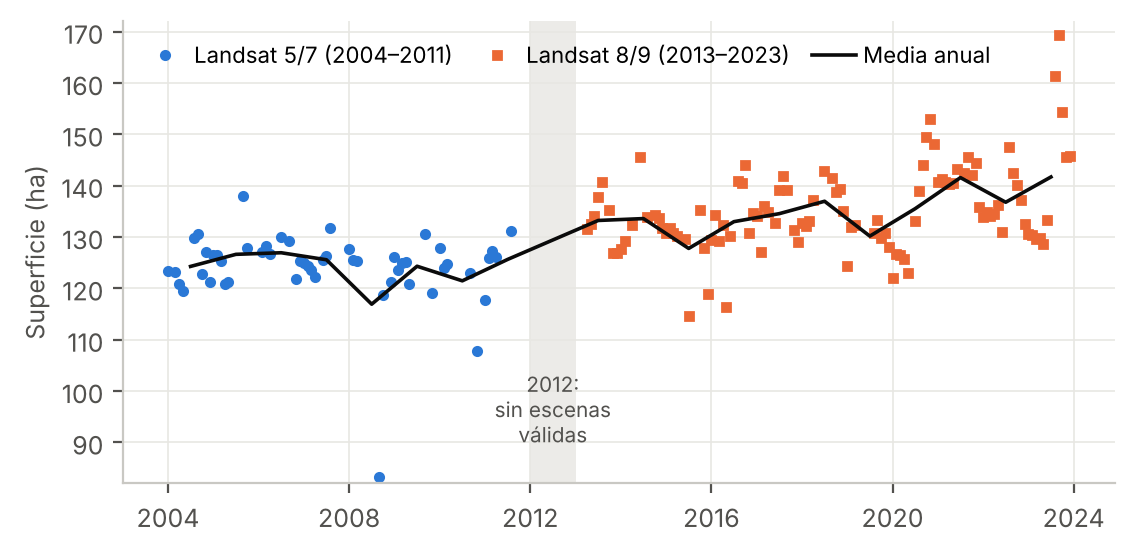
\includegraphics[width=\textwidth]{fig/f1_serie_mensual.png}
\caption{Área mensual observada de la Laguna Torca, 2004--2023 (160 meses con dato; no se imputó ningún valor). Colores y símbolos distinguen la época de sensor. Línea negra: media de los meses observados de cada año.}
\label{fig:serie}
\end{figure}

En 2004--2023 la superficie mensual observada tiene media de 131.6 ha, con un mínimo de 83.2 ha (septiembre de 2008) y un máximo de 169.4 ha (septiembre de 2023). La Figura~\ref{fig:serie} y la Tabla~\ref{tab:anual} muestran dos regímenes distintos:

\begin{itemize}
\item \textbf{2004--2011 (Landsat 5/7):} media mensual de 124.1 ha (desviación 7.2 ha, 96 meses), sin tendencia (tau $=-0.07$, $p=0.91$; pendiente $-0.20$ ha/año).
\item \textbf{2013--2023 (Landsat 8/9):} media mensual de 135.3 ha (desviación 8.2 ha, 132 meses), con tendencia creciente de $+0.94$ ha/año (tau $=0.60$, $p=0.01$), más marcada en 2020--2023 (media 2020--2024: 139.3 ha).
\end{itemize}
La diferencia de 11.2 ha entre épocas (${\approx}9\,\%$) es estadísticamente muy significativa (Mann--Whitney, $p<0.001$), pero coincide exactamente con el cambio de sensor, por lo que \textbf{no puede interpretarse como un aumento real de la laguna} sin una calibración cruzada entre sensores (ver Limitaciones). La variación anual es irregular: las anomalías anuales van de $-11.6$ ha (2008) a $+12.2$ ha (2023), y los cambios de un año al siguiente oscilan entre $-7.9$ y $+8.1$ ha.

La \textbf{variación mensual neta} entre meses consecutivos con dato (124 pares en 2004--2023) tiene promedio $-0.32$ ha, desviación estándar de 5.9 ha y mediana del valor absoluto de 2.6 ha: la laguna cambia en un mes típico unas pocas hectáreas, sin una dirección predominante. Los promedios por mes calendario se apoyan en entre 4 y 16 pares y no son concluyentes; el patrón estacional se describe mejor con la Figura~\ref{fig:estacional}.

\begin{table}[H]
\centering
\caption{Superficie anual de la Laguna Torca, 2004--2023 (años con al menos 3 meses observados). La anomalía es respecto de la climatología mensual de toda la serie; la variación es el cambio de la anomalía respecto del año anterior (no se calcula en 2013 porque 2012 no tiene datos).}
\label{tab:anual}
\small
\begin{tabular}{rrrrrl}
\toprule
Año & Meses obs. & Área media (ha) & Anomalía (ha) & Variación (ha) & Sensor \\
\midrule
2004 & 9 & 124.2 & $-$5.4 & 1.9 & L5/L7 \\
2005 & 7 & 126.6 & $-$1.7 & 3.7 & L5/L7 \\
2006 & 7 & 126.9 & $-$1.5 & 0.1 & L5/L7 \\
2007 & 7 & 125.5 & $-$3.7 & $-$2.2 & L5/L7 \\
2008 & 6 & 116.9 & $-$11.6 & $-$7.9 & L5/L7 \\
2009 & 7 & 124.3 & $-$3.5 & 8.1 & L5/L7 \\
2010 & 5 & 121.4 & $-$6.6 & $-$3.1 & L5/L7 \\
2011 & 5 & 125.6 & $-$2.8 & 3.7 & L5/L7 \\
2013 & 8 & 133.2 & 2.8 & -- & L8/L9 \\
2014 & 8 & 133.6 & 4.0 & 1.2 & L8/L9 \\
2015 & 9 & 127.8 & $-$0.8 & $-$4.8 & L8/L9 \\
2016 & 11 & 133.0 & 3.5 & 4.2 & L8/L9 \\
2017 & 10 & 134.5 & 5.1 & 1.6 & L8/L9 \\
2018 & 9 & 136.9 & 8.4 & 3.3 & L8/L9 \\
2019 & 8 & 130.2 & 0.5 & $-$7.9 & L8/L9 \\
2020 & 11 & 135.5 & 6.2 & 5.7 & L8/L9 \\
2021 & 11 & 141.6 & 12.1 & 5.8 & L8/L9 \\
2022 & 11 & 136.8 & 7.3 & $-$4.8 & L8/L9 \\
2023 & 11 & 141.7 & 12.2 & 4.9 & L8/L9 \\
\bottomrule
\end{tabular}
\end{table}


\subsection{Pregunta 2: estacionalidad, puntos de quiebre y anomalías}

\paragraph{Estacionalidad.} Una vez descontada la diferencia de nivel entre épocas, los 12 meses del año no tienen la misma superficie (Kruskal--Wallis, $H=35.2$, 11 grados de libertad, $p=0.0002$). Agosto, septiembre y octubre están por encima de la media de su época (+6.8, +4.5 y +3.6 ha), compatible con la recarga invernal, mientras que mayo queda 5.0 ha por debajo (Figura~\ref{fig:estacional}). La amplitud estacional (${\approx}\pm5$ ha, cerca del 4\,\% del área) es pequeña frente al salto entre sensores, y los meses de invierno (mayo a julio) tienen pocas observaciones por la nubosidad (7 a 9 por mes).

\begin{figure}[H]
\centering
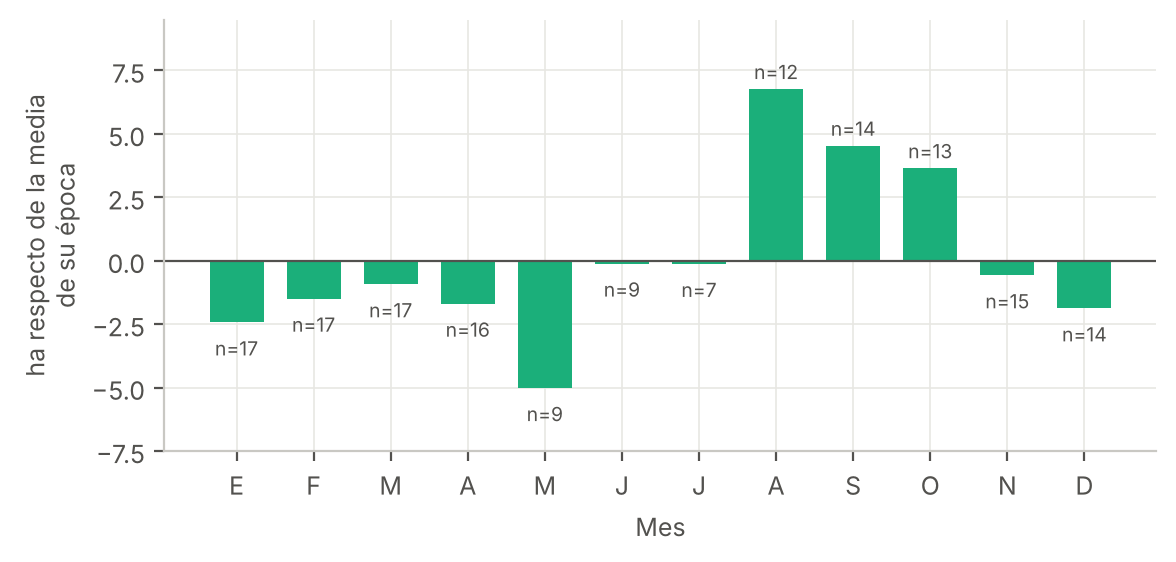
\includegraphics[width=0.92\textwidth]{fig/f3_estacionalidad.png}
\caption{Diferencia media del área de cada mes respecto de la media de su época de sensor, 2004--2023. Sobre cada barra, el número de meses observados.}
\label{fig:estacional}
\end{figure}

\paragraph{Puntos de quiebre.} El test de Pettitt sobre las anomalías anuales 2004--2023 detecta un quiebre tras 2011 ($p=0.003$; anomalía media $-4.6$ ha antes y $+5.6$ ha después). Con toda la serie (1985--2024) el resultado es el mismo (quiebre tras 2011, $p<0.001$; $-5.2$ ha antes y $+6.0$ ha después). \textbf{Ese año es justamente el cambio de Landsat 5/7 a Landsat 8/9}, de modo que el único punto de quiebre significativo de la serie es indistinguible de un artefacto del sensor (Figura~\ref{fig:anomalia}). No se detectó un segundo quiebre dentro de ninguna de las dos épocas, pero con 8 y 11 años por época la potencia de la prueba es baja.

\begin{figure}[H]
\centering
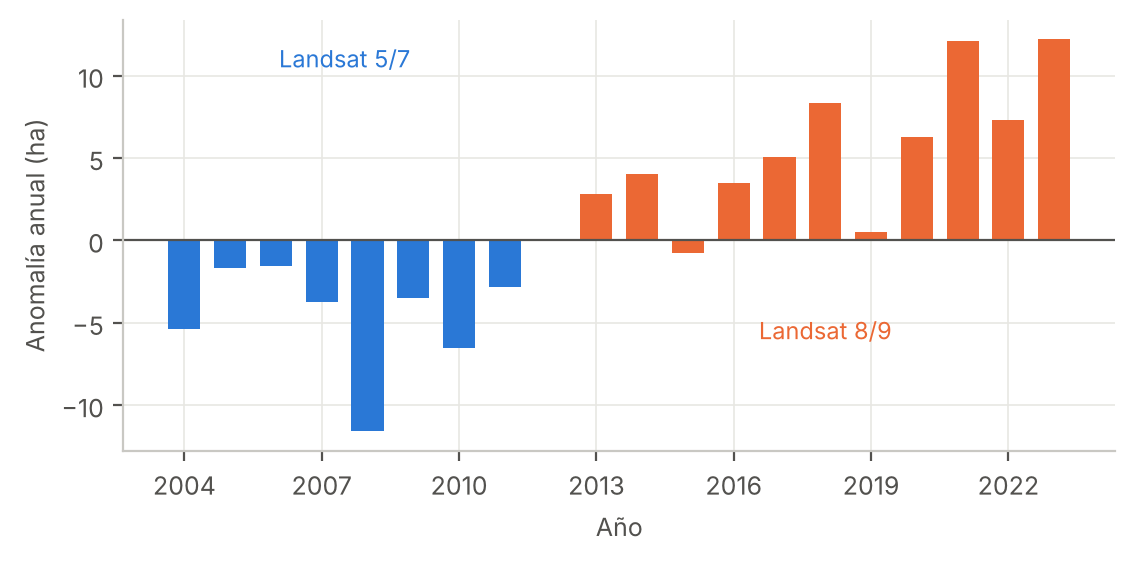
\includegraphics[width=0.92\textwidth]{fig/f2_anomalia_anual.png}
\caption{Anomalía anual del área respecto de la climatología mensual de toda la serie (solo años con al menos 3 meses observados).}
\label{fig:anomalia}
\end{figure}

\paragraph{Anomalías.} Se marcaron los meses cuyo área se aleja más de 2.5 desviaciones estándar ($\sigma=6.8$ ha) de lo esperado para su época y su mes. Son cinco, todos en 2004--2023:

\begin{center}
\begin{tabular}{lrl}
\toprule
Mes & Anomalía (ha) & Lectura \\
\midrule
Septiembre de 2008 & $-45.6$ & Posible error (nube o sombra); revisar \\
Julio de 2015 & $-22.4$ & Posible error o evento puntual; revisar \\
Noviembre de 2020 & $+17.4$ & A revisar \\
Agosto de 2023 & $+18.3$ & Compatible con un invierno lluvioso \\
Septiembre de 2023 & $+28.5$ & Compatible con un invierno lluvioso \\
\bottomrule
\end{tabular}
\end{center}
Las dos anomalías negativas son lo bastante bruscas como para sospechar un error de medición no capturado por las reglas de curación. Para 2023 el clima CR2MET no está disponible (termina en 2019), por lo que la causa climática de los meses altos no pudo verificarse.

\subsection{Pregunta 3: correlación con precipitación y temperatura}

La Tabla~\ref{tab:corr} y la Figura~\ref{fig:corr} muestran que la correlación ``cruda'' (hasta 0.34 en valor absoluto) está inflada por dos efectos que no tienen que ver con el clima: el ciclo estacional compartido y el salto de sensor. Al exigir lo que realmente pregunta el proyecto (¿cuando llueve más de lo normal, la laguna es más grande de lo normal \emph{dentro de una misma época de sensor}?), la correlación cae a valores entre $-0.05$ y $0.18$. La única asociación estadísticamente significativa es con la precipitación acumulada de 3 meses ($\rho=0.18$, $p=0.010$), que explica en torno al 3\,\% de la varianza. Los valores-$p$ no consideran la autocorrelación de las series, por lo que son optimistas. Con la temperatura, el signo cambia de una versión a otra (por ejemplo, la temperatura máxima pasa de $-0.25$ a $+0.18$ y luego a $-0.05$), señal de que no hay una relación estable.

\begin{table}[H]
\centering
\caption{Correlación de Spearman entre el área y el clima (208 meses, 1985--2019). La relevante es la última versión, que descuenta el ciclo estacional y la diferencia de época de sensor; $R^2\approx\rho^2$.}
\label{tab:corr}
\small
\begin{tabular}{lrrrrr}
\toprule
Variable & $\rho$ cruda & $\rho$ sin ciclo & $\rho$ sin ciclo ni época & Valor-$p$ & $R^2$ (\%) \\
\midrule
Precipitación del mes & 0.27 & 0.06 & 0.11 & 0.105 & 1.3 \\
Precipitación, rezago 1 mes & 0.33 & 0.08 & 0.09 & 0.225 & 0.7 \\
Precipitación, rezago 2 meses & 0.28 & $-$0.01 & 0.09 & 0.197 & 0.8 \\
Precipitación acumulada 3 meses & 0.34 & 0.08 & 0.18 & 0.010 & 3.2 \\
Precipitación acumulada 12 meses & $-$0.17 & $-$0.16 & 0.08 & 0.254 & 0.6 \\
Temperatura máxima & $-$0.25 & 0.18 & $-$0.05 & 0.442 & 0.3 \\
Temperatura mínima & $-$0.33 & 0.12 & $-$0.05 & 0.442 & 0.3 \\
\bottomrule
\end{tabular}
\end{table}


\begin{figure}[H]
\centering
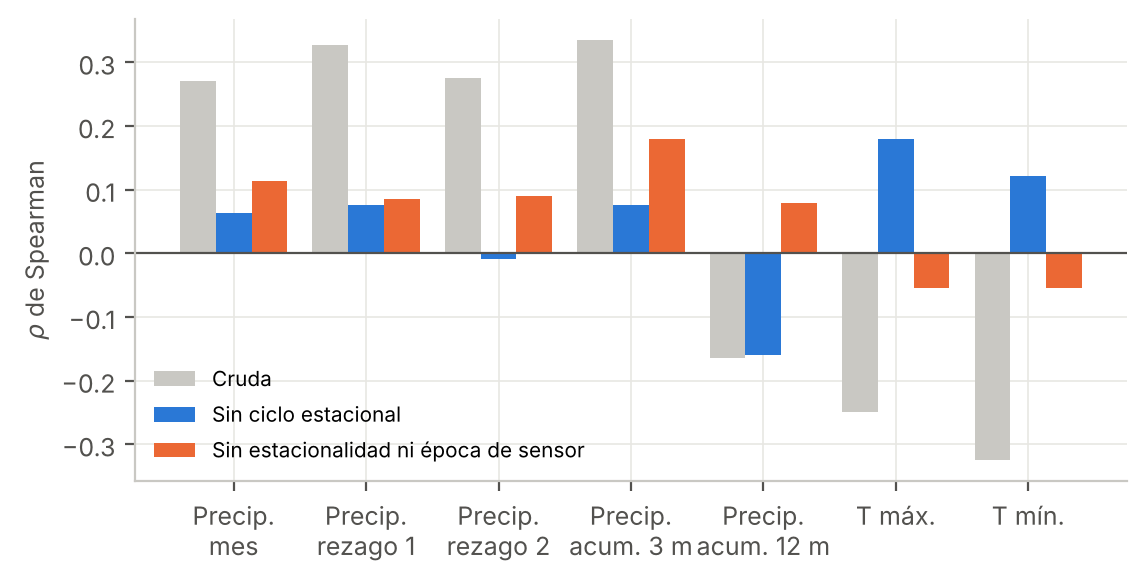
\includegraphics[width=0.92\textwidth]{fig/f4_correlaciones.png}
\caption{Correlación de Spearman entre el área y cada variable climática, en tres versiones (208 meses, 1985--2019).}
\label{fig:corr}
\end{figure}

\subsection{Pregunta 5: ¿qué modelo de pronóstico tiene el menor error?}

La Tabla~\ref{tab:cv} y la Figura~\ref{fig:cv} comparan todos los modelos en el mismo esquema de validación. El \textbf{menor RMSE lo obtiene Ridge con clima (7.68 ha)}, pero queda esencialmente empatado con Ridge sin clima (7.70), SARIMAX sin clima (7.75) y la persistencia del último valor observado (7.82 ha): las diferencias (0.02 a 0.14 ha) son más de diez veces menores que la desviación estándar del RMSE entre pliegues (cercana a 2 ha). Tres hechos acotan lo que se puede concluir:

\begin{itemize}
\item \textbf{La ganancia sobre la climatología mensual (${\approx}19\,\%$) proviene de la variable \texttt{epoca}}, es decir, del salto de nivel del sensor, no del clima.
\item \textbf{El clima no mejora a ningún modelo de forma consistente.} Con el mismo modelo, agregar las variables climáticas cambia el RMSE en $-0.02$ ha (Ridge), $-0.04$ (Random Forest), $+0.20$ (XGBoost) y $+0.12$ (SARIMAX); un valor positivo significa que empeora.
\item \textbf{Una vez retirados el ciclo estacional y el efecto de sensor (Tabla~\ref{tab:cvB}), ningún modelo supera a predecir la media}: Ridge con clima obtiene 6.93 ha contra 6.91 ha de la media, y XGBoost con clima empeora a 7.46 ha.
\end{itemize}
Además, los dos primeros bloques de entrenamiento (hasta 2006 y hasta enero de 2010) no contienen ninguna escena Landsat 8/9, por lo que los modelos no pueden aprender el salto de sensor hasta el tercer pliegue. En consecuencia, \textbf{el modelo más robusto es Ridge con estacionalidad y época de sensor}, que logra un error comparable al mejor con la menor complejidad; el modelo con clima se conserva solo porque la propuesta exige proyectar con escenarios climáticos.

\begin{table}[H]
\centering
\caption{Validación cruzada temporal, objetivo: nivel del área (4 pliegues de 24 meses); RMSE, desviación del RMSE entre pliegues y MAE en ha. ``Ganancia'' es la reducción del RMSE respecto de la climatología mensual. ``Sin clima'' incluye estacionalidad y época de sensor.}
\label{tab:cv}
\small
\begin{tabular}{lrrrr}
\toprule
Modelo & RMSE & Desv. RMSE & MAE & Ganancia (\%) \\
\midrule
Ridge (+ clima) & 7.68 & 2.09 & 5.58 & 19.6 \\
Ridge (sin clima) & 7.70 & 2.17 & 5.60 & 19.4 \\
SARIMAX(1,0,0) (sin clima) & 7.75 & 2.25 & 5.37 & 18.9 \\
Persistencia (referencia) & 7.82 & 2.24 & 5.65 & 18.2 \\
SARIMAX(1,0,0) (+ clima) & 7.87 & 2.46 & 5.67 & 17.7 \\
Random Forest (+ clima) & 7.92 & 1.99 & 5.53 & 17.1 \\
Random Forest (sin clima) & 7.96 & 1.78 & 5.49 & 16.7 \\
XGBoost (sin clima) & 8.04 & 1.71 & 5.59 & 15.9 \\
XGBoost (+ clima) & 8.24 & 1.74 & 5.61 & 13.8 \\
Media (referencia) & 9.38 & 0.37 & 7.27 & 1.8 \\
Climatología mensual (referencia) & 9.56 & 0.59 & 7.55 & 0.0 \\
\bottomrule
\end{tabular}
\end{table}


\begin{figure}[H]
\centering
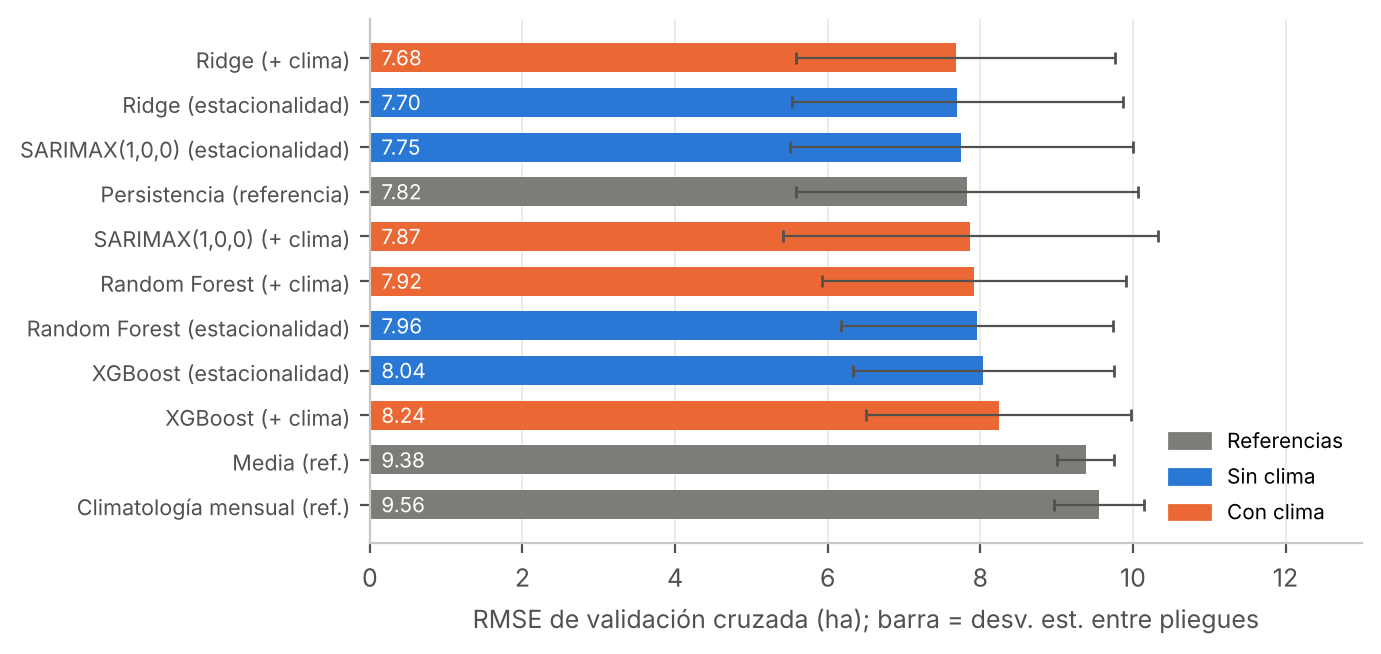
\includegraphics[width=0.95\textwidth]{fig/f5_rmse_modelos.png}
\caption{RMSE de validación cruzada temporal para el nivel del área (hectáreas). Las barras de error son la desviación estándar entre los 4 pliegues.}
\label{fig:cv}
\end{figure}

\begin{table}[H]
\centering
\caption{Validación cruzada temporal, objetivo: anomalía del área sin ciclo estacional ni efecto de época (aísla la señal climática del salto de sensor); mismas columnas que la tabla anterior.}
\label{tab:cvB}
\small
\begin{tabular}{lrrrr}
\toprule
Modelo & RMSE & Desv. RMSE & MAE & Ganancia (\%) \\
\midrule
Media (referencia) & 6.91 & 2.01 & 4.48 & 3.5 \\
Ridge (sin clima) & 6.92 & 2.15 & 4.49 & 3.4 \\
Ridge (+ clima) & 6.93 & 2.27 & 4.53 & 3.2 \\
Random Forest (+ clima) & 7.13 & 2.09 & 4.73 & 0.5 \\
Random Forest (sin clima) & 7.15 & 2.18 & 4.68 & 0.2 \\
Climatología mensual (referencia) & 7.16 & 2.20 & 4.69 & 0.0 \\
XGBoost (sin clima) & 7.19 & 2.19 & 4.75 & $-$0.4 \\
XGBoost (+ clima) & 7.46 & 1.99 & 4.90 & $-$4.1 \\
Persistencia (referencia) & 8.48 & 2.24 & 5.81 & $-$18.4 \\
\bottomrule
\end{tabular}
\end{table}


\subsection{Pregunta 4: superficie proyectada a corto y mediano plazo}

Se proyectó el área con el modelo Ridge con clima para cada uno de los modelos globales de los dos escenarios, con \texttt{epoca}\,$=1$ (escala de Landsat 8/9), y se comparó con una \emph{corrida de control} que usa clima constante (climatología 1986--2005). La Tabla~\ref{tab:proy} y la Figura~\ref{fig:proy} muestran que la superficie proyectada es prácticamente plana: \textbf{${\approx}133$ ha en todos los horizontes y en ambos escenarios}, igual a la corrida de control (133.18 ha). La diferencia entre RCP~8.5 y RCP~2.6 no pasa de 0.22 ha, y el efecto del cambio climático respecto del control no supera 0.17 ha en valor absoluto, frente a un error de validación de 7.7 ha. Para el corto plazo (2025--2040) la proyección es de 133.2 ha (RCP~2.6) y 133.1 ha (RCP~8.5); para el mediano plazo (2041--2070), 133.2 y 133.1 ha.

Esta estabilidad no es evidencia de que la laguna vaya a permanecer estable: es la consecuencia directa de que el modelo casi no usa el clima (secciones anteriores). Dos observaciones refuerzan la cautela: el nivel proyectado queda 2 ha por debajo de la media de Landsat 8/9 (135.3 ha) y 6 ha por debajo de la media observada en 2020--2024 (139.3 ha), y la banda de $\pm7.7$ ha de la figura es solo un orden de magnitud del error, no un intervalo de predicción formal. Una variante mensual con imputación MICE y suavizado da diferencias entre escenarios de hasta $-0.56$ ha en el largo plazo, también menores que 1 ha. El modelo anual con MICE del notebook original, en cambio, sí produce diferencias grandes (hasta 22 ha); se analiza en la sección~\ref{sec:mice}.

\begin{table}[H]
\centering
\caption{Superficie proyectada (ha) por escenario y horizonte: media de los modelos globales, rango entre el percentil 10 y 90 de los modelos, y diferencia respecto de la corrida de control (133.18 ha).}
\label{tab:proy}
\small
\begin{tabular}{llrrr}
\toprule
Escenario & Horizonte & Media & P10--P90 & Efecto vs. control \\
\midrule
RCP~26 & Corto (2025--2040) & 133.16 & 132.85--133.36 & $-$0.02 \\
RCP~26 & Mediano (2041--2070) & 133.16 & 132.97--133.39 & $-$0.01 \\
RCP~26 & Largo (2071--2095) & 133.23 & 132.93--133.52 & 0.05 \\
RCP~85 & Corto (2025--2040) & 133.10 & 132.81--133.44 & $-$0.08 \\
RCP~85 & Mediano (2041--2070) & 133.05 & 132.72--133.38 & $-$0.12 \\
RCP~85 & Largo (2071--2095) & 133.01 & 132.67--133.45 & $-$0.17 \\
\bottomrule
\end{tabular}
\end{table}


\begin{figure}[H]
\centering
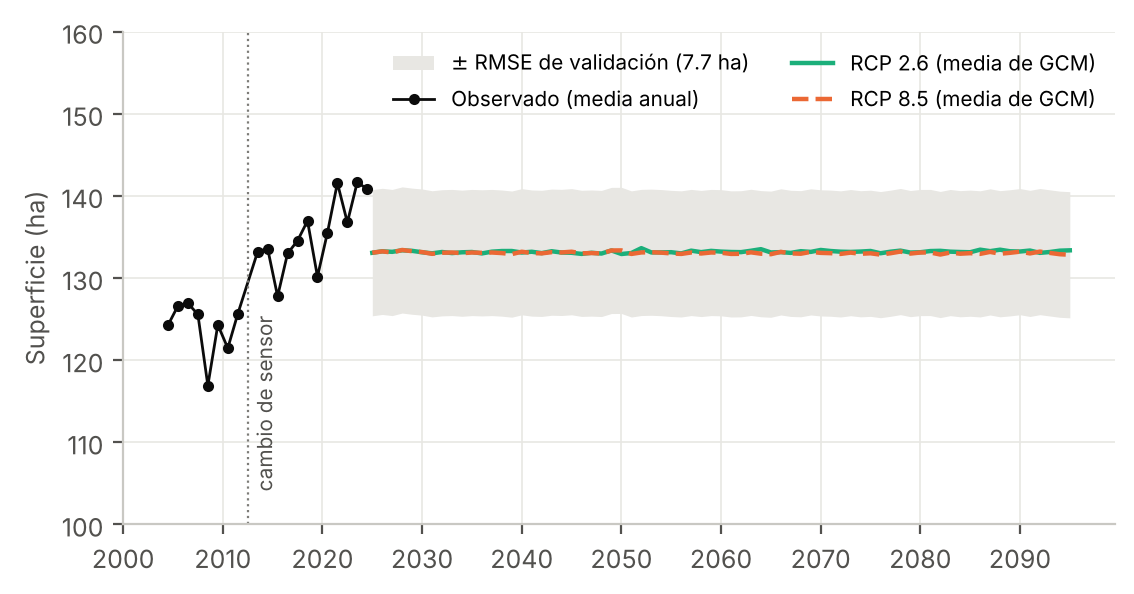
\includegraphics[width=0.95\textwidth]{fig/f6_proyeccion.png}
\caption{Promedio anual observado y proyección 2025--2095 (media entre modelos globales) bajo RCP~2.6 y RCP~8.5. La banda gris es $\pm$ el RMSE de validación; no es un intervalo de predicción.}
\label{fig:proy}
\end{figure}

\section{Modelo anual con imputación MICE (modelo del notebook original)}
\label{sec:mice}

El notebook original incluía un segundo modelo que sí mostraba diferencias claras entre escenarios climáticos. Se reconstruyó con los datos de este proyecto y se evaluó con la misma exigencia que los demás. Esta sección explica cómo funciona, qué resultados da y por qué esos resultados no se sostienen.

\subsection{Descripción del modelo}

\begin{itemize}
\item \textbf{Serie objetivo:} promedio anual del área mensual \emph{imputada} con MICE (Random Forest, usando el clima del mismo mes) y luego \emph{suavizada} con un filtro Savitzky--Golay (ventana de 13 meses, polinomio de grado 3), 1985--2019. La Figura~\ref{fig:reconstruida} muestra esta serie: el suavizado convierte los 208 meses observados entre 1985 y 2019 en una curva continua de 420 meses cuyos valores anuales varían solo entre 118.9 y 135.8 ha.
\item \textbf{Predictores:} precipitación, temperatura máxima y temperatura mínima, promediadas por año, con rezagos de hasta 2 años para la precipitación y 1 año para las temperaturas (7 variables: P, P1, P2, Tx, Tx1, Tn, Tn1).
\item \textbf{Modelo:} regresión lineal ajustada con 33 años (1987--2019), proyectada modelo global por modelo global con una media móvil de 3 años.
\end{itemize}
Se presentan tres versiones:
\begin{enumerate}
\item \textbf{Original:} como en el notebook original. El índice de precipitación futura del CR2 se suma en milímetros a la línea base, y las columnas de precipitación y temperaturas de los modelos globales se emparejan por posición, no por nombre.
\item \textbf{Corregido:} las columnas se emparejan por nombre de modelo global, y la precipitación futura se calcula como línea base multiplicada por el índice dividido por 100 (los archivos de precipitación del CR2 están normalizados: su promedio 1986--2005 es 100 en todos los modelos, no son milímetros).
\item \textbf{Corregido + época:} además se agrega la variable \texttt{epoca}, para que el salto entre sensores no se confunda con el clima.
\end{enumerate}

\begin{figure}[H]
\centering
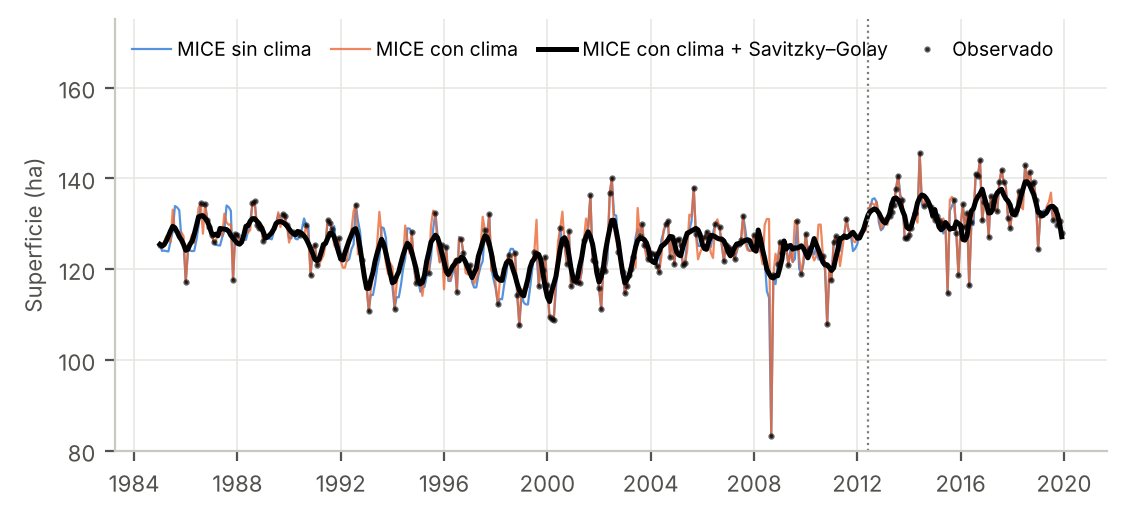
\includegraphics[width=\textwidth]{fig/f10_serie_reconstruida.png}
\caption{Serie reconstruida con MICE (ajuste con toda la muestra, solo ilustrativo). Los puntos negros son los meses realmente observados; la línea gruesa es la serie que usa el modelo anual, con oscilaciones regulares producidas por la imputación y el suavizado.}
\label{fig:reconstruida}
\end{figure}

\subsection{Resultados: sí hay diferencia entre escenarios}

La Tabla~\ref{tab:mdif} y las Figuras~\ref{fig:mice} y~\ref{fig:dif} muestran que el modelo original proyecta una superficie mucho mayor bajo RCP~8.5 que bajo RCP~2.6, y que la diferencia crece con el horizonte: 3.3 ha en el corto plazo, 9.9 ha en el mediano y 21.9 ha en el largo plazo. La versión corregida da casi lo mismo (2.2, 8.6 y 20.1 ha). En cambio, el modelo mensual con datos observados (sección~\ref{sec:resultados}) da diferencias de $-0.1$ a $-0.2$ ha. La versión con época de sensor reduce la diferencia a 0.2, 0.8 y 1.9 ha, por debajo del error de validación.

Hay tres señales de alarma en el modelo original:
\begin{itemize}
\item Bajo RCP~8.5 el índice de precipitación futura es el más bajo (84.4, frente a 96.0 en RCP~2.6, con 100 como referencia histórica) y la temperatura sube más, pero el modelo predice \emph{más} superficie de agua. Es lo contrario de lo que cabría esperar hidrológicamente.
\item En la versión original solo se emparejan 12 de los 26 modelos globales de RCP~2.6 y 31 de los 39 de RCP~8.5 (por el emparejamiento por posición), y los niveles proyectados (106 a 108 ha en RCP~2.6) quedan más de 30 ha por debajo de lo observado en 2020--2024 (139.3 ha).
\item La precipitación de entrada sumada como milímetros llega a unos 143 mm/mes, fuera del rango con que se entrenó el modelo (18 a 80 mm/mes).
\end{itemize}

\begin{table}[H]
\centering
\caption{Superficie proyectada (ha) por el modelo anual con MICE, en sus tres versiones, y diferencia entre escenarios. Las últimas filas repiten el modelo mensual con datos observados.}
\label{tab:mdif}
\small
\begin{tabular}{llrrr}
\toprule
Modelo & Horizonte & RCP~2.6 & RCP~8.5 & RCP~8.5 $-$ RCP~2.6 \\
\midrule
Original & Corto (2025--2040) & 106.1 & 109.4 & 3.3 \\
Original & Mediano (2041--2070) & 107.9 & 117.8 & 9.9 \\
Original & Largo (2071--2095) & 108.0 & 129.9 & 21.9 \\
Corregido & Corto (2025--2040) & 132.0 & 134.3 & 2.2 \\
Corregido & Mediano (2041--2070) & 134.3 & 142.9 & 8.6 \\
Corregido & Largo (2071--2095) & 134.6 & 154.8 & 20.1 \\
Corregido + época & Corto (2025--2040) & 133.4 & 133.6 & 0.2 \\
Corregido + época & Mediano (2041--2070) & 133.7 & 134.5 & 0.8 \\
Corregido + época & Largo (2071--2095) & 133.8 & 135.7 & 1.9 \\
Mensual observado (sección~\ref{sec:resultados}) & Corto (2025--2040) & 133.2 & 133.1 & $-$0.1 \\
Mensual observado (sección~\ref{sec:resultados}) & Mediano (2041--2070) & 133.2 & 133.1 & $-$0.1 \\
Mensual observado (sección~\ref{sec:resultados}) & Largo (2071--2095) & 133.2 & 133.0 & $-$0.2 \\
\bottomrule
\end{tabular}
\end{table}


\begin{figure}[H]
\centering
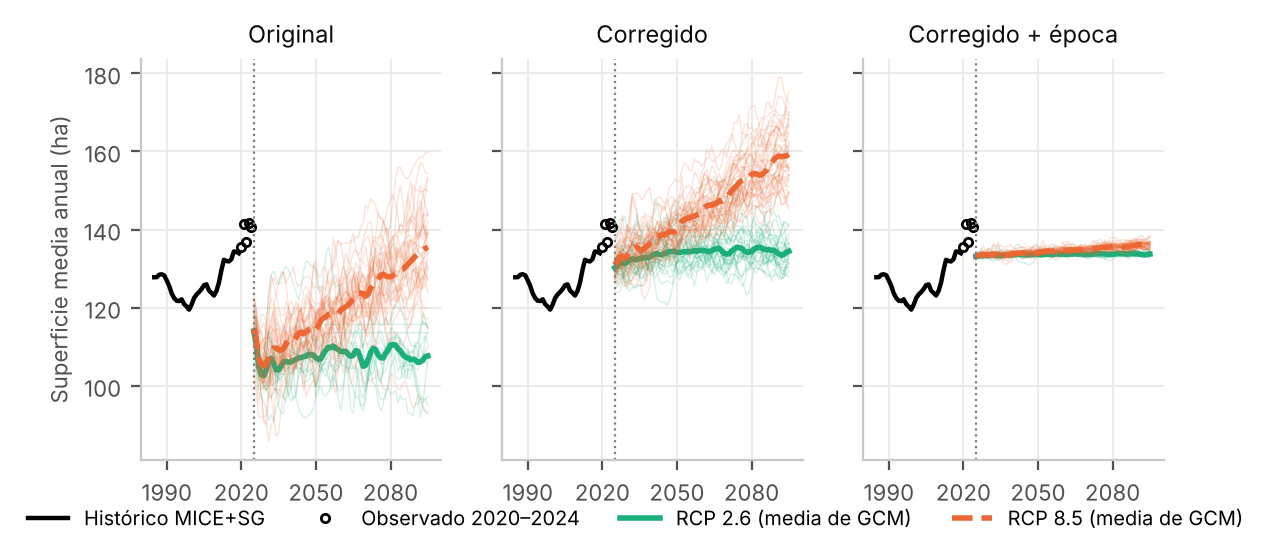
\includegraphics[width=\textwidth]{fig/f7_modelo_anual_mice.png}
\caption{Proyección del modelo anual con MICE bajo RCP~2.6 y RCP~8.5, en sus tres versiones. Las líneas finas son los modelos globales individuales; las gruesas, su media. Los círculos son el promedio anual observado en 2020--2024 (sin imputar).}
\label{fig:mice}
\end{figure}

\begin{figure}[H]
\centering
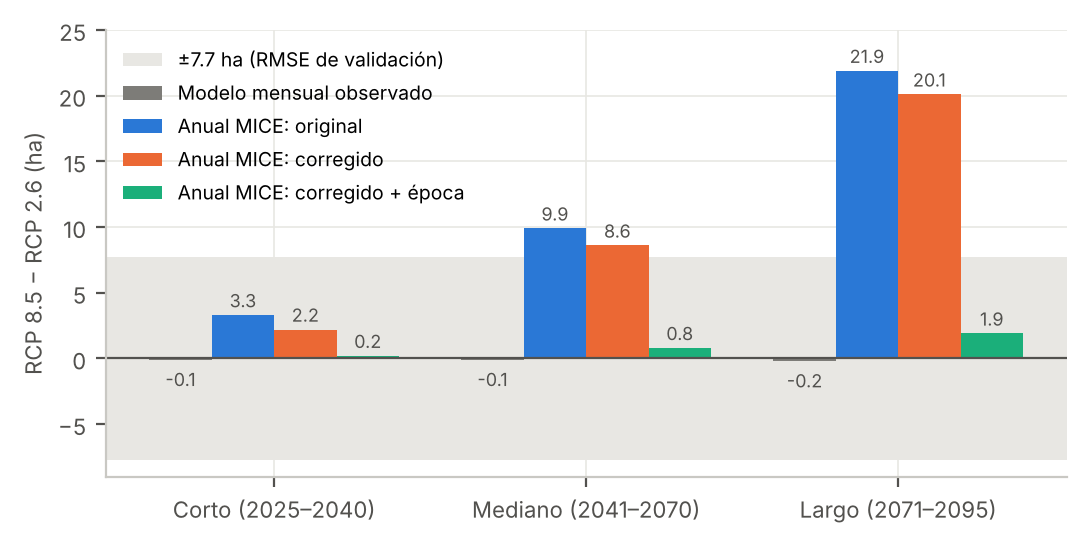
\includegraphics[width=0.92\textwidth]{fig/f9_diferencia_escenarios.png}
\caption{Diferencia entre escenarios (RCP~8.5 menos RCP~2.6) según el modelo. La banda gris es el RMSE de validación del modelo mensual ($\pm7.7$ ha).}
\label{fig:dif}
\end{figure}

\subsection{De dónde sale la diferencia}

\paragraph{Variables que la producen.} La Figura~\ref{fig:contrib} descompone la diferencia de 2071--2095 por variable (coeficiente por diferencia de la variable entre escenarios). La precipitación aporta apenas 2.5 ha de las 20.1. El resto viene de las temperaturas, con efectos de signo opuesto que casi se cancelan: la temperatura mínima del año anterior suma $+21.5$ ha y la máxima del año anterior resta 12.4 ha. Los coeficientes (Tabla~\ref{tab:mcoef}) son $+12.2$ ha/$^\circ$C para la mínima y $-6.3$ ha/$^\circ$C para la máxima, dos variables correlacionadas entre sí ($r=0.68$); coeficientes grandes y de signo contrario en variables colineales son un síntoma típico de sobreajuste, no de un mecanismo físico.

\paragraph{Extrapolación.} En el entrenamiento la temperatura anual varía muy poco (máxima entre 18.7 y 20.3\,$^\circ$C; mínima entre 6.7 y 8.2\,$^\circ$C). Bajo RCP~8.5 en 2071--2095 las medias proyectadas son 22.4 y 10.1\,$^\circ$C, unos 2 $^\circ$C por encima de cualquier valor visto, de modo que los coeficientes se extrapolan lejos del rango donde se estimaron.

\paragraph{Cambio de sensor.} El área sube desde 2013, el mismo año del cambio de sensor, y la temperatura también tiende a subir. Sin una variable de sensor, el modelo usa el calentamiento como sustituto de ese escalón. Al agregar \texttt{epoca} (coeficiente $+8.7$ ha), el $R^2$ dentro de la muestra pasa de 0.26 a 0.64, los coeficientes de temperatura se reducen a una fracción y la diferencia entre escenarios cae de 20.1 a 1.9 ha.

\begin{figure}[H]
\centering
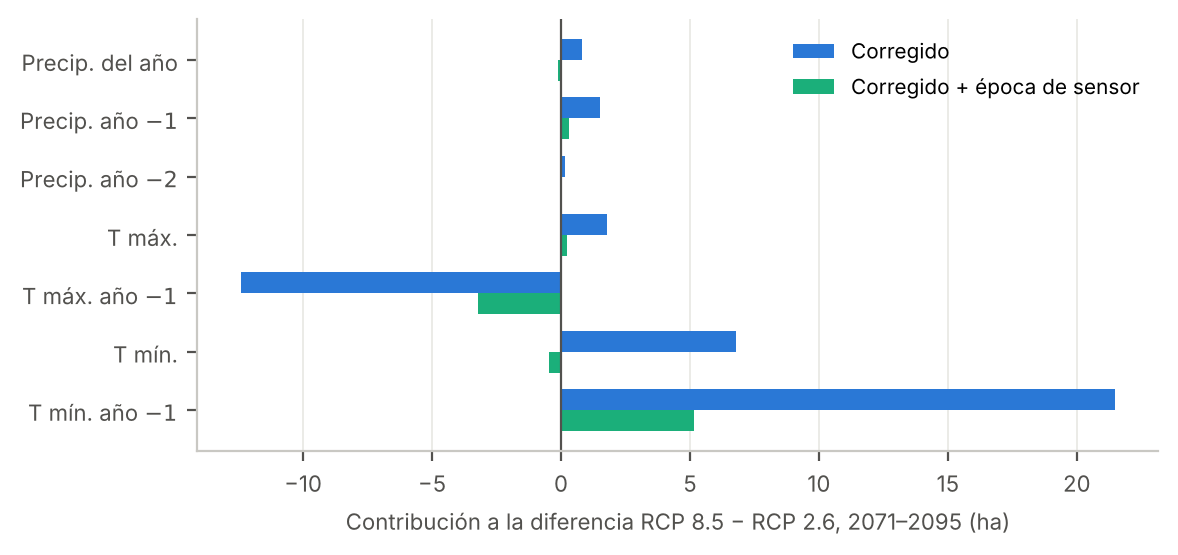
\includegraphics[width=0.92\textwidth]{fig/f8_contribucion_variables.png}
\caption{Contribución de cada variable a la diferencia entre RCP~8.5 y RCP~2.6 en 2071--2095, en el modelo corregido sin y con la variable de época.}
\label{fig:contrib}
\end{figure}

\begin{table}[H]
\centering
\caption{Coeficientes del modelo lineal anual (ha por mm/mes de precipitación o por $^\circ$C). $R^2$ dentro de la muestra: 0.26 (original) y 0.64 (con época).}
\label{tab:mcoef}
\small
\begin{tabular}{lrr}
\toprule
Variable & Original (7 variables) & Con época de sensor \\
\midrule
Precipitación del año & $-$0.09 & 0.01 \\
Precipitación año $-1$ & $-$0.17 & $-$0.03 \\
Precipitación año $-2$ & $-$0.02 & 0.00 \\
Temperatura máxima & 0.90 & 0.12 \\
Temperatura máxima año $-1$ & $-$6.30 & $-$1.64 \\
Temperatura mínima & 3.80 & $-$0.25 \\
Temperatura mínima año $-1$ & 12.22 & 2.93 \\
Época de sensor (0/1) & -- & 8.66 \\
\bottomrule
\end{tabular}
\end{table}


\subsection{Validación del modelo anual}

Se validó hacia adelante: para cada año de 2002 a 2019, el modelo se ajusta con los años anteriores y se predice ese año (Tabla~\ref{tab:mval}). Contra el área \emph{realmente observada}, el modelo lineal original tiene un RMSE de 6.56 ha, \textbf{peor que la media histórica} (5.91 ha) y que repetir el año anterior (4.51 ha). Con la variable de época mejora a 5.32 ha: supera por poco a la media pero no a la persistencia. Contra la serie MICE+SG el error parece menor (5.34 ha), porque esa serie es suave y se parece a sí misma de un año a otro, que es la ilusión descrita en la sección~\ref{sec:antecedente}.

\begin{table}[H]
\centering
\caption{Validación hacia adelante del modelo anual, 2002--2019 (RMSE en ha; 17 años contra lo observado y 18 contra la serie MICE+SG).}
\label{tab:mval}
\small
\begin{tabular}{lrr}
\toprule
Modelo & Contra área observada & Contra serie MICE+SG \\
\midrule
Lineal original (7 variables) & 6.56 & 5.34 \\
Lineal + época & 5.32 & 3.77 \\
Media histórica (referencia) & 5.91 & 5.50 \\
Año anterior (referencia) & 4.51 & 2.45 \\
\bottomrule
\end{tabular}
\end{table}


\subsection{Lectura}

El modelo anual con MICE produce la diferencia entre escenarios que se esperaba, pero no es evidencia de un efecto climático: depende de (i) una serie objetivo imputada y suavizada, (ii) unidades de precipitación mal tratadas en la versión original, (iii) dos temperaturas colineales con coeficientes opuestos que se extrapolan fuera de rango y (iv) el salto de sensor, que se confunde con el calentamiento. Corregidos los puntos (ii) y (iv), la diferencia a 2095 pasa de 22 ha a 2 ha, equivalente a la incertidumbre del modelo, y el modelo no supera a la persistencia al validarlo con datos observados. Por eso, en este informe el modelo anual con MICE se presenta como una \textbf{reconstrucción del enfoque original y de sus limitaciones}, no como la proyección recomendada.

\section{Antecedente: el flujo de trabajo inicial y por qué se reemplazó}
\label{sec:antecedente}

El primer flujo de trabajo del proyecto (un cuaderno inicial con imputación MICE y SARIMAX) se rediseñó antes de obtener los resultados anteriores. Se documenta porque sus resultados \emph{parecían} mejores y la diferencia es una lección metodológica.

\begin{table}[H]
\centering
\caption{Flujo inicial frente al flujo final.}
\label{tab:flujos}
\small
\begin{tabular}{p{3.0cm}p{5.8cm}p{5.8cm}}
\toprule
 & Flujo inicial & Flujo final \\
\midrule
Clima histórico & Tres planillas con 108 meses de precipitación (2014--2024) y 57 de temperatura (2015--2020); el resto se rellenaba con el promedio & CR2MET v2.0 completo, 1979--2019 \\
Meses sin área & Imputados con MICE (Random Forest, 30 iteraciones), usando el clima del mismo mes, y suavizados con Savitzky--Golay (ventana de 13 meses, grado 3, centrado) & No se imputa; se usan solo meses observados \\
Modelo & SARIMAX(1,0,1)(1,0,1)$_{12}$ con 6 regresores; una versión anual con Ridge y un conjunto de 63 modelos globales & Referencias, Ridge, SARIMAX(1,0,0), Random Forest y XGBoost \\
Validación & Último 20\,\% de la serie ya imputada y suavizada & Validación cruzada temporal solo sobre meses observados \\
Proyección & Proyecciones del CR2 en una escala distinta a la del entrenamiento (de ahí valores de 600 a 1\,200 ha) & Método delta por modelo, con corrida de control \\
\bottomrule
\end{tabular}
\end{table}

Tres problemas hacían engañosos los resultados iniciales:
\begin{enumerate}
\item \textbf{Clima mayormente inventado.} Más de tres cuartas partes de los meses de precipitación y casi nueve de cada diez de temperatura (sobre 480 meses, 1985--2024) se completaban con el promedio, de modo que el modelo aprendía de un clima casi constante.
\item \textbf{Imputación circular.} En una réplica del flujo inicial, MICE con el clima del mismo mes produce áreas ``correlacionadas'' con la lluvia por construcción: en los meses imputados la correlación con la precipitación de 3 meses es de $0.21$ ($p=0.002$, 212 meses), mientras que sin usar el clima en la imputación es de $-0.04$ ($p=0.53$); en los meses realmente observados es de $0.17$. La relación que el satélite nunca midió aparece sola.
\item \textbf{Error medido contra la serie propia.} En una réplica del flujo inicial (MICE y suavizado, con Ridge y clima), evaluada contra su propia serie imputada y suavizada, se obtiene un RMSE de 4.13 ha; evaluada solo contra los meses realmente observados es de 7.44 ha. El error aparente era ${\approx}44\,\%$ menor que el real. Por su parte, el suavizado centrado usa meses futuros, lo que filtra información hacia la validación.
\end{enumerate}
Un cuarto problema, la \emph{desalineación de escala} entre la precipitación mensual de entrenamiento y las proyecciones del CR2 (índice normalizado), se detalla en la sección~\ref{sec:mice}.

\section{Cumplimiento de los objetivos}

\begin{table}[H]
\centering
\caption{Objetivos específicos del proyecto y su estado.}
\label{tab:obj}
\small
\begin{tabular}{p{4.4cm}p{2.7cm}p{7.2cm}}
\toprule
Objetivo & Estado & Evidencia y salvedades \\
\midrule
1. Preprocesar imágenes 2004--2023 (nubes, ruido) & Cumplido & Máscara \texttt{QA\_PIXEL}, nubosidad $<20\,\%$, SLC-off y cinco reglas de curación (sección 2.2). Sin corrección atmosférica propia (se usa reflectancia de superficie USGS). \\
2. Segmentación e índices espectrales (NDWI/MNDWI) & Parcial & NDWI con umbral $>0$. No se implementó MNDWI ni otro método de segmentación, y no se midió la exactitud contra una referencia. \\
3. Serie histórica, tendencias y anomalías & Cumplido, con reserva & Series mensual y anual, Kendall, Theil--Sen, Pettitt, Kruskal--Wallis y anomalías (secciones 3.1 y 3.2). El quiebre coincide con el cambio de sensor. \\
4. Correlacionar con datos meteorológicos & Cumplido & Spearman en tres versiones con CR2MET (208 meses). Asociación débil ($\rho\le0.18$). \\
5. Entrenar modelos clásicos y de ML & Cumplido & Media, climatología, persistencia, Ridge, SARIMAX, Random Forest y XGBoost, con y sin clima; proyección a 2095. \\
6. Evaluar con RMSE/MAE y validación temporal; elegir el más robusto & Cumplido, sin ganador claro & Validación cruzada de ventana expansiva. Ridge es el más robusto, pero empata con la persistencia (diferencia dentro del ruido). \\
\bottomrule
\end{tabular}
\end{table}


\section{Limitaciones}

\begin{enumerate}
\item \textbf{Salto de sensor confundido con la señal.} La diferencia de 11 ha entre Landsat 5/7 y 8/9 y el único quiebre significativo coinciden con el cambio de sensor. No se calibraron los sensores con pares de escenas casi simultáneas (en 2012 no hay escenas válidas, por lo que no existe solapamiento directo en la serie curada). Mientras no se haga, la tendencia posterior a 2013 no puede atribuirse con seguridad al clima ni al sensor.
\item \textbf{Cobertura irregular.} Solo el 67\,\% de los meses de 2004--2023 tiene dato, con menos observaciones en invierno, justo cuando la laguna cambia más.
\item \textbf{Clima solo hasta 2019.} CR2MET no cubre los últimos cuatro años de la serie (2020--2024), que incluyen los valores más altos del área.
\item \textbf{Clima mensual de baja resolución.} CR2MET es una grilla (0.05$^\circ$) derivada en parte de reanálisis; no captura la hidrología local (aportes de caudales, extracciones, manejo del humedal, nivel freático), que probablemente explica gran parte de la variación del área.
\item \textbf{Muestra pequeña para validar.} Con 4 pliegues de 24 meses, la desviación entre pliegues (${\approx}2$ ha) es mayor que cualquier diferencia entre los mejores modelos.
\item \textbf{Proyección sin respaldo estadístico.} Las proyecciones dependen de un modelo que no demostró capacidad predictiva superior a la persistencia, y los escenarios RCP son una variable independiente de lo que ocurra con el uso del suelo y del agua.
\item \textbf{Sin verificación en terreno.} El umbral NDWI y las reglas de curación no se validaron contra imágenes de mayor resolución ni mediciones de nivel.
\end{enumerate}

\section{Conclusiones}

\begin{enumerate}
\item La superficie de la Laguna Torca en 2004--2023 oscila alrededor de 132 ha (media mensual 131.6 ha), con un mínimo de 83.2 ha y un máximo de 169.4 ha. Los valores anuales van de 116.9 ha (2008) a 141.7 ha (2023).
\item Existe un ciclo estacional pequeño pero significativo (agosto a octubre más extenso). El único quiebre significativo (tras 2011) coincide con el cambio de sensor Landsat, por lo que \textbf{no hay evidencia suficiente de un cambio hidrológico} en el periodo.
\item La asociación estadística con la precipitación y la temperatura, una vez controlados el ciclo estacional y el sensor, es débil (máximo $\rho=0.18$, $R^2\approx3\,\%$).
\item Ningún modelo (clásico o de Machine Learning) supera de forma clara a la persistencia ni a un Ridge simple; el clima no mejora el pronóstico. El modelo más robusto es Ridge con estacionalidad y época de sensor (RMSE 7.7 ha, MAE 5.6 ha).
\item Las proyecciones a 2095 bajo RCP~2.6 y RCP~8.5 son casi iguales (${\approx}133$ ha) y deben tratarse como una prueba de sensibilidad. El modelo anual con MICE del notebook original muestra una diferencia de unas 22 ha, pero se explica por temperaturas colineales extrapoladas y por el salto de sensor, y no supera a la media en validación (con la variable de época cae a 2 ha). La principal ruta de mejora no es un algoritmo más complejo, sino \textbf{calibrar los sensores, incorporar clima posterior a 2019 y datos hidrológicos locales}.
\end{enumerate}

\begin{thebibliography}{9}
\bibitem{cr2met} Centro de Ciencia del Clima y la Resiliencia (CR2). \emph{Producto grillado CR2MET v2.0 de precipitación y temperatura para Chile} y \emph{Explorador de Simulaciones Climáticas}. \url{https://www.cr2.cl}. % VERIFICAR: completar la cita formal con el autor y versión que indica el CR2.
\bibitem{garreaud2017} Garreaud, R. D., et al. (2017). The 2010--2015 megadrought in central Chile: impacts on regional hydroclimate and vegetation. \emph{Hydrology and Earth System Sciences}, 21, 6307--6327.
\bibitem{gorelick2017} Gorelick, N., Hancher, M., Dixon, M., Ilyushchenko, S., Thau, D., \& Moore, R. (2017). Google Earth Engine: planetary-scale geospatial analysis for everyone. \emph{Remote Sensing of Environment}, 202, 18--27.
\bibitem{hyndman2021} Hyndman, R. J., \& Athanasopoulos, G. (2021). \emph{Forecasting: Principles and Practice} (3.\textordfeminine{} ed.). OTexts.
\bibitem{mcfeeters1996} McFeeters, S. K. (1996). The use of the Normalized Difference Water Index (NDWI) in the delineation of open water features. \emph{International Journal of Remote Sensing}, 17(7), 1425--1432.
\bibitem{pettitt1979} Pettitt, A. N. (1979). A non-parametric approach to the change-point problem. \emph{Journal of the Royal Statistical Society: Series C (Applied Statistics)}, 28(2), 126--135.
\bibitem{sen1968} Sen, P. K. (1968). Estimates of the regression coefficient based on Kendall's tau. \emph{Journal of the American Statistical Association}, 63(324), 1379--1389.
\bibitem{vanvuuren2011} van Vuuren, D. P., et al. (2011). The representative concentration pathways: an overview. \emph{Climatic Change}, 109, 5--31.
\end{thebibliography}

\end{document}
